\chapter{Asking Denver Millionaires How Much Money They Make}

This chapter is best read as a bookkeeping exercise in commercial reasoning. We are first shown outcomes in the form of striking money figures, and only afterward are we allowed to ask what kinds of businesses, skills, habits, and social structures make such figures possible. The lecture is not a blackboard derivation, but it does contain a real mathematical payload: we must distinguish annual personal income from company revenue, separate scale from profit, and track the causal chain from skills to offers, from networks to belief, and from recurring revenue to acquisition economics.

\section{Money Shock and Framing}

The lecture opens with a deliberate shock: several annual money figures are thrown at us before any scene-setting occurs. We should not smooth this away. The point of the opening is to place scale in front of mechanism.

\begin{definition}
We distinguish three objects throughout:
\begin{itemize}
\item \(Y\): annual personal income;
\item \(R\): annual business or company revenue;
\item \(P\): profit.
\end{itemize}
The opening montage mixes these objects, and part of the discipline of the notes is to keep them separate.
\end{definition}

A cautious transcription of the opening claims is
\begin{align}
Y_{\max}^{(1)} &> \$10\,\mathrm{M}, &
Y_{\max}^{(2)} &= \$1.4\,\mathrm{M}, \\
Y_{\max}^{(3)} &= \$1.7\,\mathrm{M}, &
Y_{\max}^{(4)} &= \$1.2\,\mathrm{M},
\end{align}
followed by company-level figures,
\begin{align}
R_{\max}^{(\mathrm{company})} &= \$30\,\mathrm{M}, &
R^{(\mathrm{ecom})} &= \$50\,\mathrm{M}.
\end{align}

Already the lecture is forcing a distinction. A person may report what he made in a year, while another reports what one of his companies generated in revenue. These are not interchangeable magnitudes. If we collapse them, we lose the structure of the interview at the first step.

\begin{remark}
The opening numbers are unattributed in montage form. For our purposes they are best treated as anonymous evidence of scale rather than as carefully assigned identities.
\end{remark}

\section{Industries, Vehicles, and Business Scale}

Only after the money shock does the host reset the scene in Denver and ask the first explanatory question: what industry did you pursue? This is the right next move. Wealth, in the lecture, is not a substance; it is attached to vehicles.

The answers are varied but concrete: one interviewee moves from thirteen years as a pastor into coaching and consulting, travels and speaks, and sits on the boards of eight companies. Another names internet marketing. Another combines digital marketing with real estate, specifying Airbnb on the real-estate side and coaching people into Airbnb on the digital side. Another names a fitness coaching company with fifty coaches. Another names a short-form content agency working with large influencers at a scale of roughly four thousand videos per month.

We may record the explicit scale markers as
\begin{align}
t_{\mathrm{pastor}} &= 13\,\mathrm{years}, &
N_{\mathrm{boards}} &= 8, \\
N_{\mathrm{coaches}} &= 50, &
V_{\mathrm{month}} &\approx 4000.
\end{align}

What matters in this section is the variety of operating forms. The lecture does not present one canonical wealth machine. It presents consulting, coaching, board participation, marketing, real estate, fitness services, media production, and e-commerce. The first lesson is therefore structural: the path to scale is not unique, but each path has a definite commercial object.

\section{Advice to the Younger Self: Time, Identity, and Sales}

The lecture now pivots from biography to principle. Instead of asking only what the speakers do, it asks what they would tell a younger version of themselves. This is where the interview starts extracting durable mechanisms from lived history.

One speaker says that his younger self would not have listened, then identifies the real deficit: not courage exactly, but time. One must take time to find oneself rather than merely climb other people's mountains. The lecture is careful here. It is not saying that ambition is false; it is saying that borrowed ambition is unstable.

A second strand of advice is persistence. ``Keep going'' appears not as a slogan but as a correction to the inevitable temptation to stop once friction appears. A third strand is delayed gratification: early shortcuts may appear to accelerate progress, but later they return as structural weakness. In the language of the lecture, they cause more problems than good, and a brand worth keeping does not appear overnight.

Finally the section culminates in sales. Several interviewees treat sales not as one occupation among others, but as a portable competence. The claim is not subtle: learn sales early, because selling accelerates both business results and the broader ability to communicate with people.

We can summarize the logic in the mild schematic
\begin{equation}
\text{communication skill} \;\Longrightarrow\; \text{selling ability} \;\Longrightarrow\; \text{income flexibility}.
\end{equation}
The interview does not prove this formally, but it returns to it often enough that it functions as one of the lecture's governing claims.

\section{Starting a Business: Focus, Failure, and Horizons}

Once the lecture has extracted principles from hindsight, it turns practical: what is the best advice for someone starting a business now?

The first answer is focus. Internet marketers, we are told, are especially vulnerable to distraction by the next attractive product. The lecture opposes this with concentration on one specific product, followed by depth rather than restless scanning. The next answer is immediate action: jump in, dive in, and stop dabbling from a distance. Then comes a more important correction. Failure at the beginning is not evidence that the attempt was mistaken; it is part of the normal entry cost of doing anything new.

The lecture also imposes explicit time horizons. One should know the six-month, one-year, and five-year goals, and one should reward oneself along the way. In notation,
\begin{equation}
T_{\mathrm{goals}}=\{6\ \mathrm{months},\,1\ \mathrm{year},\,5\ \mathrm{years}\}.
\end{equation}
The point is not simply to dream at several scales. The point is to avoid the two common entrepreneurial distortions: impatience in the short run and vagueness in the long run.

A compact reconstruction of the section is
\begin{equation}
\text{focus} + \text{time in the game} + \text{tolerated failure}
\;\Longrightarrow\; \text{usable experience}.
\end{equation}
This is not a theorem; it is the lecture's process rule.

\section{What Remains When the Bank Account Hits Zero?}

Here the lecture reaches its sharpest conceptual hinge. The host asks what one would do if the bank account hit zero tomorrow. This is the right stress test, because it removes accumulated cash and asks what part of wealth is genuinely portable.

\subsection{Question \& Answer}

\paragraph{Question.}
If the bank balance falls to zero, what remains of the wealth-building machine?

\paragraph{Answer.}
What remains, according to the interview, is not money but structure: skills, knowledge, expertise, the ability to identify problems, access to financing, the ability to package an offer, and the ability to sell.

Let
\begin{equation}
B_0 = 0,
\qquad
K=\{\text{skills},\,\text{knowledge},\,\text{expertise}\}.
\end{equation}
One answer in the lecture is then reconstructed by the chain
\begin{align}
B_0 &= 0, \\
K &> 0, \\
K &\longrightarrow O \longrightarrow G \longrightarrow \text{cash flow},
\end{align}
where \(O\) is a commercial offer and \(G\) is a gap or problem that some client needs solved.

This deserves to be read step by step.

\begin{enumerate}
\item Set the stress test: there is no liquid cash.
\item Notice what has not vanished: the person still possesses \(K\).
\item Convert \(K\) into something saleable, namely an offer \(O\).
\item Attach \(O\) to a real need \(G\) in the market.
\item Once \(G\) is solved for a client, cash flow reappears.
\end{enumerate}

A second answer uses financing:
\begin{equation}
B_0=0,\qquad F>0 \;\Longrightarrow\; F \longrightarrow \text{operating capacity} \longrightarrow P.
\end{equation}
Here \(F\) stands for external financing. The lecture does not give a balance-sheet derivation, but the commercial logic is clear: if one can obtain capital, one can reopen the business, operate, and attempt to convert financing into profit.

A third answer is more social and more entrepreneurial. One throws a party, listens for recurring pain points, identifies the largest problems in the room, and creates a product around the repeated complaint. A fourth answer is even leaner: call friends with high-ticket offers and sell on their behalf. In both cases, the interview is saying the same thing. Wealth survives as capability before it survives as cash.

\begin{figure}
\centering
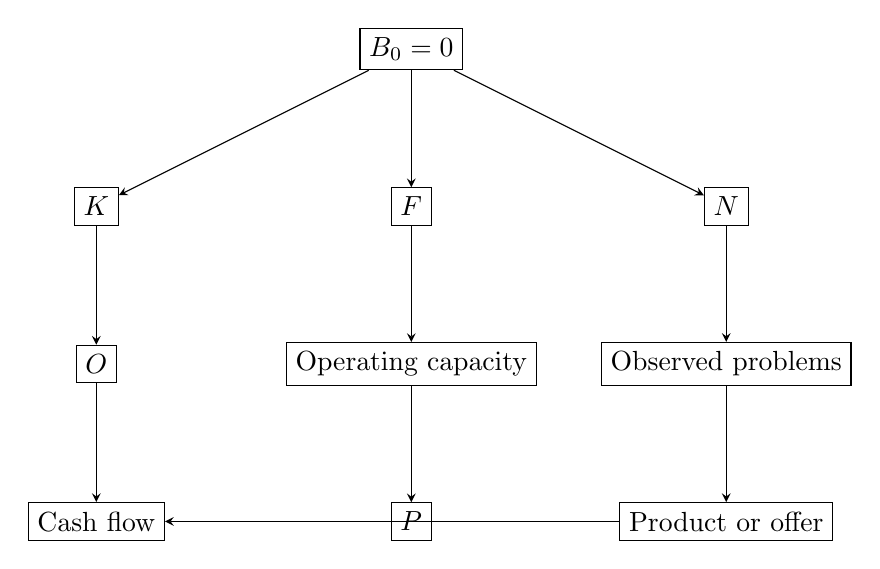
\begin{tikzpicture}[>=stealth]
\node[draw, rectangle] (b0) at (0,0) {$B_0=0$};
\node[draw, rectangle] (k) at (-4,-2) {$K$};
\node[draw, rectangle] (f) at (0,-2) {$F$};
\node[draw, rectangle] (n) at (4,-2) {$N$};

\node[draw, rectangle] (o) at (-4,-4) {$O$};
\node[draw, rectangle] (cap) at (0,-4) {Operating capacity};
\node[draw, rectangle] (prob) at (4,-4) {Observed problems};

\node[draw, rectangle] (cash) at (-4,-6) {Cash flow};
\node[draw, rectangle] (profit) at (0,-6) {$P$};
\node[draw, rectangle] (prod) at (4,-6) {Product or offer};

\draw[->] (b0) -- (k);
\draw[->] (b0) -- (f);
\draw[->] (b0) -- (n);

\draw[->] (k) -- (o);
\draw[->] (o) -- (cash);

\draw[->] (f) -- (cap);
\draw[->] (cap) -- (profit);

\draw[->] (n) -- (prob);
\draw[->] (prob) -- (prod);
\draw[->] (prod) -- (cash);
\end{tikzpicture}
\end{figure}

The diagram is not quoted from the lecture; it is a cautious reconstruction of the three main answers to the zero-balance problem.

\section{Rooms, Masterminds, and the Expansion of Belief}

The lecture next widens the frame. Once we have identified portable individual capital, we are asked about the importance of being around the right people.

Here the answers become socially precise. Good relationships are not treated as ornamental encouragement. They are accountability structures. They hold a person to his declared identity, his vision, his standards as a family man or as a business operator. They also create a kind of healthy competition. One speaker says, in effect, that one is not meant to be an island unto oneself.

A second mechanism is epistemic. When one sits at a table where others report the numbers they are doing and the ways in which their lives changed, larger outcomes stop looking imaginary. The room changes the possibility set. What had seemed abstract becomes real.

We may write the causal claim as
\begin{equation}
N_{\mathrm{quality}} \uparrow
\;\Longrightarrow\;
B_{\mathrm{belief}} \uparrow
\;\Longrightarrow\;
X_{\mathrm{execution}} \uparrow,
\end{equation}
where \(N_{\mathrm{quality}}\) measures the quality of the room or network, \(B_{\mathrm{belief}}\) the range of outcomes one can genuinely imagine as attainable, and \(X_{\mathrm{execution}}\) the corresponding range of action.

The lecture gives a concrete example. A speaker says his businesses used to stop at roughly seven figures. Then a mastermind produced a jump, and the next year brought a ten-million-dollar result. The crucial words are not merely that there was advice, but that they were able to see the potential and thereby eliminate self-limiting beliefs. The room does not do the work for you. It alters what work you are capable of imagining and therefore attempting.

\section{Sales, Personal Brand, and Recurring Revenue}

The closing movement of the lecture is the most operational. It asks for the secret to sales and then for the logic of scale in the present business environment.

The first answer is psychological but practical: be okay with rejection. Rejection is not merely pain; it is information. Hence the next rule: take more reps. In the lecture this appears through sales calls, and the claim can be written schematically as
\begin{equation}
n_{\mathrm{calls}} \uparrow
\;\Longrightarrow\;
n_{\mathrm{reps}} \uparrow
\;\Longrightarrow\;
p_{\mathrm{close}} \uparrow.
\end{equation}
We should not overstate the precision of this relation, but the operating idea is clear. Repetition improves pitch, communication, and calm under resistance.

The next answer is result-first selling. One interviewee explicitly ties his agency's scale to leading with results rather than with image. If the results are not there, he says he is willing to have the uncomfortable conversation that the fit is wrong. This is a disciplined statement about credibility. Sales is not treated here as verbal pressure; it is treated as the commercialization of demonstrated outcomes.

The final and most mathematical idea is recurring revenue. Once the lecture asks how a business really scales, recurring revenue appears as a change in acquisition logic. If a customer produces value over time, then the firm does not need the first transaction to carry the whole weight of profitability.

Let \(\mathrm{CAC}\) be customer acquisition cost and \(\mathrm{LTV}\) customer lifetime value. Then the relevant quantity is
\begin{equation}
\Pi_{\mathrm{customer}}=\mathrm{LTV}-\mathrm{CAC}.
\end{equation}
A business with recurring revenue can tolerate an initial acquisition loss provided the total economics over the customer lifetime remain favorable.

A simple reconstruction makes this explicit. Suppose the acquisition period loses \(|\pi_0|\), but recurring gross contribution of \(m_t\) arrives over time. Then
\begin{align}
\Pi_{\mathrm{customer}}
&= -|\pi_0| + \sum_{t=1}^{T} m_t, \\
&\approx -|\pi_0| + Tm
\qquad
\text{if } m_t \approx m.
\end{align}
Therefore,
\begin{equation}
\Pi_{\mathrm{customer}} > 0
\;\Longrightarrow\;
\text{an initially unprofitable acquisition can still be rational.}
\end{equation}

This is exactly the point made in the lecture: one can sometimes acquire at a loss, because one is not demanding that the first sale produce the entire profit. One can therefore outspend a competitor who is forced to make money immediately. The lecture does not give retention curves or a detailed unit-economics model, but its logic is unmistakable:
\begin{equation}
RR \uparrow
\;\Longrightarrow\;
\mathrm{LTV} \uparrow
\;\Longrightarrow\;
\mathrm{CAC}_{\max} \uparrow.
\end{equation}

The surrounding advice fits cleanly inside this logic. Build a personal brand. Develop content. Become comfortable on camera. Keep speaking until it feels natural. Put out free value consistently. All of these are acquisition and trust mechanisms. Recurring revenue then determines how aggressively those mechanisms can be funded.

\section{Summary}

The lecture begins with money as spectacle and ends with money as structure. We first encounter annual income and revenue figures, then trace them back to industries, skills, identity, patience, focus, and sales. The central question---what remains when the bank account hits zero?---reveals the lecture's deepest claim: wealth is not only stored cash, but also portable capability, network position, and commercial judgment. By the end, recurring revenue supplies the final piece of rigor. Once lifetime value exceeds acquisition cost, scale becomes a numbers game of a very particular kind, and the interview has completed its movement from headline figures to operating logic.